\documentclass{article}

\usepackage{graphicx}

\graphicspath{./}

\begin{document}
    \title  { \textbf{SYSC 4602 Assignment 4} }
    \author {
        David Song (101071234)\\
        Ghassan Arnouk (101078550)\\
        Zachary Porter (101069001)
    }

    \maketitle

    \clearpage
    \section*{Part 3: 802.11 Physical Layer}
    \subsection*{1}
    The channel frequency is 2462 Hz.
    \subsection*{2}
    The rates used are as follows in Mbps:
    \begin{itemize}
        \item 1.0
        \item 6.0
        \item 12.0
        \item 24.0
        \item 24.0
        \item 36.0
        \item 48.0
        \item 54.0
    \end{itemize}
    \subsection*{3}
    The strongest RSSI is -44 dBm \\
    The weak RSSI is -69 dBm \\
    \\
    The difference is $-44 dBm - -69 dBm = 25 dBm$. \\

    \section*{Part 4: 802.11 Link Layer}
    \subsection*{1}
    BSS ID: (Cisco-Li\_e3:e9:8d) 00:16:b6:e3:e9:8d
    \subsection*{2}
    There are 1783 data frames in the trace. In other words 47.8\% of the frames are data frames.\\
    The most common subtype of data frame is subtype 0, which make up 1743 frames.
    \subsection*{3}
    There are 557 managment frames in the trace. In other words 14.9\% of the frames are managment frames.\\
    The most common subtype of managment frame is subtype 8, which make up 458 frames.
    \subsection*{4}
    There are 1391 control frames in the trace. In other words 37.3\% of the frames are control frames.\\
    The most common subtype of control frame is subtype 13, which make up 1385 frames.
    \subsection*{5}
    \begin{figure}[htbp]
        \centering
        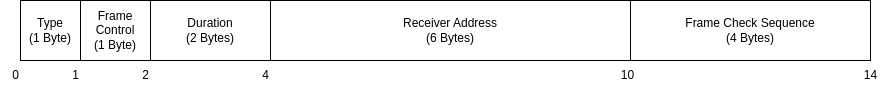
\includegraphics[width=\textwidth]{images/part4-5.drawio.png}
        \caption{Acknowledgement Frame Structure}
    \end{figure}
    \subsection*{6}
    Retransmitted frames: 1 frame
    Total frames: 3731 frames

    Retransmission rate: $1 / 3731 = 0.03\%$
    Therefore 0.03\%, or 1 out of 3731 frames that are retransmitted
    \subsection*{7}
    Power down frames: 16 frame
    Total frames: 3731 frames

    Percentage of frames sent: $16 / 3731 = 0.4\%$
    Therefore 0.4\%, or 16 out of 3731 frames that are sent signal that the client is powering down.
    \section*{Part 5: 802.11 Management}
    \subsection*{1}
        BSS ID of main AP is Cisco\_Li\_e3:e9:8d
    \subsection*{2}
        Beacon frames are sent every 0.1022 seconds approximately
    \subsection*{3}
        The main AP supports the following data rates:\\
        1, 2, 5.5, 11, 18, 24, 36, 54 [Mbit/sec]
    \subsection*{4}
        The Beacon frame transmission is sent at a rate of 1.0 Mb/s
    \subsection*{5}
        \begin{itemize}
            \item The association response frame has a type/subtype value of 0x0001
            \item The association request frame has a type/subtype value of 0x0000
        \end{itemize}
    \subsection*{6}
        \begin{itemize}
            \item The probe response frame has a type/subtype value of 0x0005
            \item The probe request frame has a type/subtype value of 0x0004
        \end{itemize}
\end{document}
